\chapter[ARQUITETURA PARA PROCESSAMENTO DE DADOS]{ARQUITETURA PARA PROCESSAMENTO DE DADOS}
\label{chapter:architecture}

A \textbf{Arquitetura Kappa} é o padrão de projeto escolhido para servir de
base para o novo serviço de processamento de dados do InterSCity. A Arquitetura
Lambda não justifica a maior complexidade no contexto atual da plataforma, de
modo que essa escolha facilita a manutenibilidade e adoção do serviço pelo
time atual do InterSCity. A Arquitetura Kappa permitirá a análise em tempo-real
sem que ocorra perda de informações relevantes, o que é importante no contexto de
cidades inteligentes, ao passo em que permite a análise de dados históricos,
desde que estes tenham sido pré-processados. Esta decisão resulta na escolha de
uma tecnologia de processamento \textit{streaming} e de um
\textit{broker} adequado.

O \textbf{Apache Spark} é a tecnologia de \textit{streaming} escolhida,
principalmente por dispor nativamente de biblioteca de clusterização e
aprendizagem de máquina. Esta ferramenta ainda facilita, caso necessário, a
troca para a Arquitetura Lambda, por dispor de processamento \textit{batch}.
O \textbf{Apache Kafka} é o \textit{broker} escolhido, sendo esta uma escolha
menos óbvia que a anterior. Embora o RabbitMQ já seja utilizado pelo
InterSCity e tenha vantagens em certos aspectos em relação ao Kafka, não
dispor de uma interface nativa que o conecte ao Spark resultou nessa decisão.
Outro fator é o gerenciamento nativo de \textit{log} por parte do
Kafka, que ajuda na implantação da Arquitetura Kappa. O Kafka, contudo, só
será utilizado no serviço de processamentos, não forçando mudanças no
ecossistema de microsserviços do InterSCity. A Figura \ref{fig:stack} ilustra
a pilha de tecnologias que deve compor a Arquitetura Kappa no InterSCity, e
as principais relações entre os serviços caso fosse utilizado a abordagem com
\textit{log}, e a Figura \ref{fig:stack2} ilustra a pilha de tecnologias caso
não fosse utilizado \textit{log}, e sim o uso explícito de produtores.

\begin{figure}
  \centering
    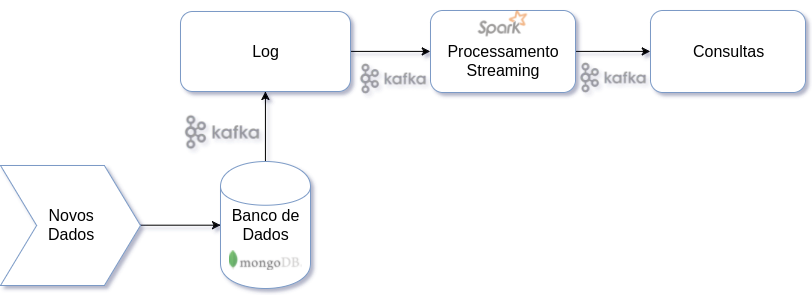
\includegraphics[scale=0.5]{figuras/kappa_tools.png}
  \caption{Pilha de tecnologias utilizadas - Apache Kafka, Apache Spark e
    MongoDB, e suas interações com o InterSCity com uso do \textit{log}.}
  \label{fig:stack}
\end{figure}

\begin{figure}
  \centering
    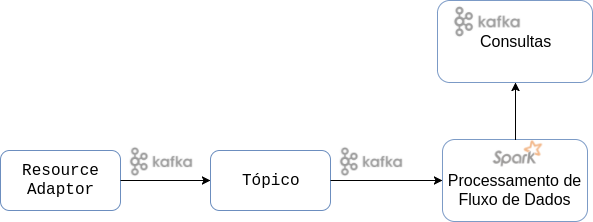
\includegraphics[scale=0.5]{figuras/kappa_tools2.png}
  \caption{Pilha de tecnologias utilizadas - Apache Kafka, Apache Spark, e suas
    interações com o InterSCity sem o uso do \textit{log}.}
  \label{fig:stack2}
\end{figure}

\section{IMPLEMENTAÇÃO}

A implementação da Arquitetura Kappa decidida foi a adaptação sem a utilização
do \textit{log}, e foi dividida em três etapas: (i) configuração do ambiente,
contemplando as ferramentas escolhidas; (ii) ligações entre os diferentes
serviços, tornando possível a publicação de mensagens no Kafka e sendo possível
seu processamento no Spark; e (iii) disponibilização de \textit{hooks} que
possam ser estendidos futuramente, possibilitando a criação de um
\textit{pipeline de dados} customizável. A implementação sem o uso de
\textit{log} foi escolhida pois seu uso apresenta maior latência, pois é
necessário que os dados sejam inseridos no banco de dados e apresentados no
\textit{log}, para que depois sejam fornecidos ao Spark. Outro motivo é que
a implementação com \textit{log} força o uso da conexão entre o \textit{log} e
o Kafka, que não conta com um conector já desenvolvido caso seja utilizada a
linguagem Python.

A implementação do novo serviço trouxe para o InterSCity o \textbf{Shock},
um componente responsável por abstrair as comunicações entre as diferentes
ferramentas, e por trazer a extensibilidade mencionada na terceira etapa da
implementação. Pseudo algoritmos presentes no apêndice \ref{appendix:impl}
ilustram o uso das ferramentas escolhidas na implementação da Arquitetura
Lambda.

\begin{figure}
  \centering
    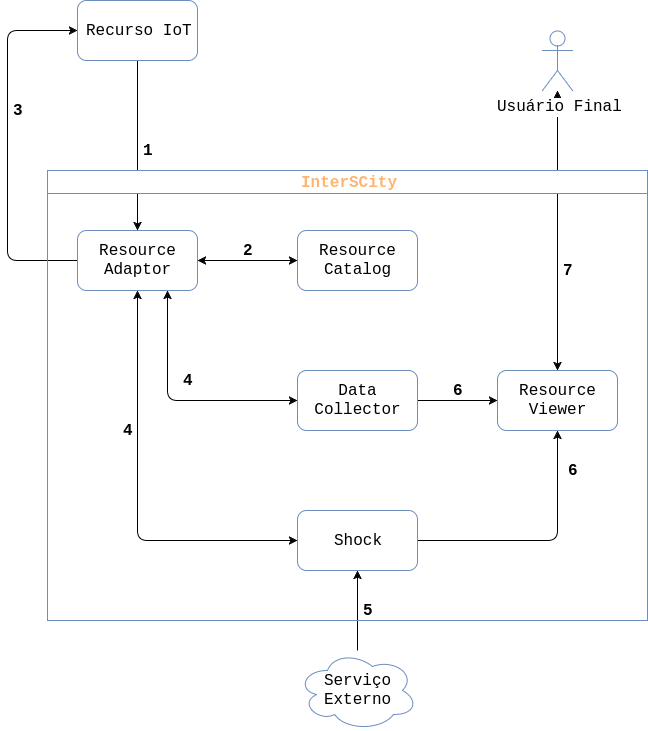
\includegraphics[scale=0.45]{figuras/shock_usage.png}
  \caption{Pilha de tecnologias utilizadas - Apache Kafka, Apache Spark, e suas
    interações com o InterSCity sem o uso do \textit{log}.}
  \label{fig:shock_usage}
\end{figure}

A Figura \ref{fig:shock_usage} ilustra um novo fluxo completo do InterSCity,
com a adição do novo serviço de processamento de dados. O início do fluxo
(passos 1 ao 3) continua o mesmo, e foi detalhado na Seção
\ref{sec:architecture}. As mudanças começam quando o (4) Resource Adaptor passa
a publicar a chegada de novos dados também no Shock através do Kafka, algo que
não trouxe grandes mudanças, mas que extendeu o InterSCity. Serviços externos
(5) anunciam no Shock quais operações devem ser executadas no \textit{stream}
de dados, de modo que os novos dados serão processados com esse conjunto de
operações. Por fim, os resultados do Shock e do Data Collector (6) serão
disponibilizados, podendo ser consumidos por aplicações como o microsserviço
Resource Viewer, que trata os dados para (7) disponibilizá-los ao usuário final.

A configuração do ambiente, assim como seguido pelo time do InterSCity, foi
guiada pelo uso de conteinêres do Docker. Uma configuração do Spark
que já havia sido desenvolvida pelo time do InterSCity foi reutilizada,
precisando de poucas mudanças. Um conteinêr com o Kafka foi configurado e
ligado aos conteinêres do Spark e do microsserviço Resource Adaptor.

A ligação entre os projetos teve início com uma adaptação no microsserviço
Resource Adaptor, que, com a mudança, passa a publicar no tópico
\textit{new\_data}, no Kafka, a atualização de novos dados. Esta
adaptação não trouxe mudanças significativas no InterSCity, não afetando o
fluxo usual da plataforma. Foi desenvolvido então o Shock, responsável por
receber mensagens em tópicos específicos do Kafka, e passá-los ao Spark
Streaming. O Shock roda \textit{micro-batches} do Spark em
intervalos de tempos definidos previamente, e em cada um destes processamentos,
\textit{hooks} extensíveis são executados. Caso queira-se anexar mais uma
tarefa no \textit{pipeline de dados}, basta então registrá-la no Shock e
fornecer uma prioridade, que define se uma tarefa deve ser executada antes ou
depois no Shock.

\section{SHOCK}

O Shock se encontra disponível em um repositório do
Gitlab\footnote{\url{https://gitlab.com/DGuedes/shock}}, e o novo microsserviço
de processamento de dados pode ser encontrado em um \textit{fork} do serviço
original\footnote{\url{https://gitlab.com/DGuedes/data-processor}}. O Shock
abstrai as configurações entre as diferentes ferramentas e pode ser customizado
por serviços externos, que definem quais operações devem ser executadas.
É configurável, possuindo um \textit{handler} para a Arquitetura Kappa
desenvolvido\footnote{\url{https://gitlab.com/DGuedes/shock/blob/master/shock/handlers.py}},
mas, caso seja desejado a implementação de um outro \textit{handler}, basta
implementar as funções obrigatórias e fornecer o novo módulo como parâmetro
para o Shock.

O Shock é utilizado da seguinte maneira: um arquivo contendo as operações a
serem executadas é disponibilizado no repositório do Shock. Este passo fornece
o controle da segurança para o servidor, que pode filtrar quem pode ou não
enviar estes arquivos, não dependendo do Shock. Após este passo, a entidade
deve solicitar ao Shock que operações disponíveis no arquivo criado sejam
executadas, através de mensagens num tópico específico do Kafka, onde o
fornecedor indica o arquivo e o nome da operação a ser executada. O Shock
então cria um novo
StreamingContext\footnote{\url{http://spark.apache.org/docs/0.7.3/api/streaming/spark/streaming/StreamingContext.html}},
adicionando as novas operações em corrente, e, por fim, inicia o novo
\textit{stream} de dados. Os próximos dados que chegarem serão então executados
pelas operações que já estavam aplicadas no Shock, e pelas novas operações
inseridas.
